\documentclass[12pt, french]{article}

\usepackage{fancyhdr, fancybox, lastpage}
\usepackage[most]{tcolorbox}
\usepackage[a4paper, margin={0.3in, .75in}]{geometry}
\usepackage{wrapfig}
\pagestyle{fancy}
\renewcommand\headrulewidth{1pt}
\renewcommand\footrulewidth{1pt}
\fancyhf{}
\rhead{ \em{Zakaria Haouzan}}
\lhead[C]{\em{Tronc Commun scientifique - option français (TCSBiof)}}
\chead[C]{}
\rfoot[C]{}
\lfoot[R]{}
\cfoot[]{\em{Page \thepage / \pageref{LastPage}}}


\newtcolorbox{Box2}[2][
enhanced, 
    breakable,
]{
                lower separated=false,
                colback=white,
colframe=white!20!black,fonttitle=\bfseries,
colbacktitle=white!30!gray,
coltitle=black,
enhanced,
attach boxed title to top left={yshift=-0.1in,xshift=0.15in},
title=#2,#1}


\begin{document}
\begin{center}
   \shadowbox {\bf{Equilibre d'un corps solide en rotation autour d'un axe fixe  }}
\end{center}
\begin{center}
   \Large{ \em{Exercices Supplémentaires}}
\end{center}

%%_________________________Exercice ! :"_________________________Exercice
   \begin{Box2}{Exercice 1 : Equilibre d'une barre   }

\begin{wrapfigure}[2]{r}{0.22\textwidth}
  \begin{center}
	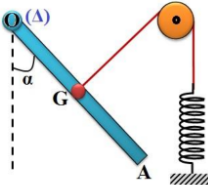
\includegraphics[width=0.22\textwidth]{./img/ex00.png}
  \end{center}
\end{wrapfigure}

Une barre (OA) homogène de masse $m = 1kg$ et de longueur L,
pouvant tourner sans frottement autour d'un axe horizontal passant
par son extrémité O, est en équilibre comme l'indique la figure.
Le fil est fixé au centre G \\de la barre, passe sur la gorge d'une
poulie et est fixé par l'autre extrémité \\à un ressort verticale de
raideur K. à l'équilibre, le fil est normal à la barre, \\avec $\alpha$= 30°.

\begin{enumerate}
	\item  Faire l’inventaire des forces appliquées sur la barre (OA) et \\les
représentées sans souci l'échelle.
\item  Ecrire l'énoncer du théorème des moments.
\item  Par application de ce théorème, trouver l'intensité de la tension du fil.
\item  déduire la valeur de la raideur du ressort sachant que son allongement à l'équilibre est $\Delta{t} = 5cm$.
\end{enumerate}
\end{Box2}


%%_________________________Exercice !2 :"_________________________Exercice
\begin{Box2}{Exercice 2 :Equilibre d'une enseigne de magasin---}

	\begin{wrapfigure}[2]{r}{0.2\textwidth}
  \begin{center}
	  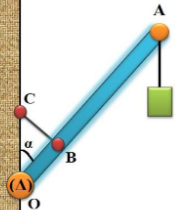
\includegraphics[width=0.2\textwidth]{./img/ex01.png}
  \end{center}
\end{wrapfigure}

Une enseigne de magasin est composée d'une barre (OA) de masse
$m=2kg$ et de longueur $L=1,20m$, capable de se mettre en rotation autour
d'un axe $(\Delta)$ horizontal et passant par le point O.

On suspend à l'aide d'un fil de masse négligeable au point A un objet
décoratif \\de masse $M = 3kg$. Et on fixe au point B qui se trouve à la
distance \\$OB =\frac{L}{4}$ du point O de l'enseigne un fil métallique BC dont
l'autre extrémité est \\fixée à un mur vertical de telle façon qu'il reste
perpendiculaire à l'enseigne.\\ L'ensemble se trouve en équilibre lorsque
$\alpha$= 30°. Avec $g = 10N/kg$.
\begin{enumerate}

	\item Faire le bilan des forces qui s’exercent sur l'objet décoratif.
	\item  Enoncer les conditions d’équilibre d’un solide soumis à deux forces.
	\item  Etudier l'équilibre de l'objet décoratif puis déduire la tension du fil au point A.
	\item  Faire le bilan des forces qui s’exercent sur l'enseigne de magasin.
	\item  Calculer l'intensité de la force exercée par le fil BC sur l'enseigne.
\end{enumerate}
\end{Box2}

%%_________________________Exercice ! 3:"_________________________Exercice
\begin{Box2}{Exercice 3 :Application  }
	\begin{wrapfigure}[2]{r}{0.25\textwidth}
  \begin{center}
	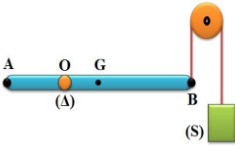
\includegraphics[width=0.25\textwidth]{./img/ex02.png}
  \end{center}
\end{wrapfigure}

On considère une tige rigide et homogène de longueur $L = AB$ et
de masse $m = 2kg$ en équilibre horizontale, et pouvant tourner
autour d'un axe horizontal fixe $(\Delta)$ passant par O.

Au point B, on fixe un fil inextensible passant par la gorge d’une
poulie et \\maintient à l'autre extrémité un corps (S) de poids $PB$.

\begin{enumerate}
	\item  Faire l’inventaire des forces appliquées sur la tige.
	\item  Quel est le poids P de la tige?
	\item  Quel doit être la valeur du poids $\vec{P_B}$ de la charge appliquée en B afin que la tige soit en équilibre?

	\item  On place une charge de poids $\vec{P_A}$ en A de $P_A = 2N$, quel doit être la nouvelle valeur de l'intensité du
 poids $\vec{P_B}$ pour que la tige soit en équilibre ?

\end{enumerate}

\textbf{Données: } $g = 10N/kg$; $AO = 40cm$; $AB = 120cm$.




\end{Box2}





%%_________________________Exercice 4 : _________________________Exercice
\begin{Box2}{Exercice 4 : Equilibre d’une pédale d'accélérateur d'automobile }

	\begin{wrapfigure}[2]{r}{0.28\textwidth}
  \begin{center}
	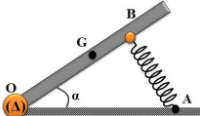
\includegraphics[width=0.28\textwidth]{./img/ex03.png}
  \end{center}
\end{wrapfigure}


La figure ci-contre schématise une pédale d'accélérateur
d'automobile. Elle est mobile autour de l'axe horizontal $(\Delta)$ passant
par le point O, le ressort AB est perpendiculaire à la pédale, la pédale
est en équilibre dans la position \\correspondant à l'angle $\alpha$ = 45°.

\begin{enumerate}
\item  Faire l’inventaire des forces appliquées sur la pédale.
\item  Quelles sont les relations existe entre ces forces à l'équilibre?
\item  Représenter ces forces sur la figure sans souci l'échelle.
\item  Déterminer la tension de T du ressort à l'équilibre .
\item  Par utilisation de la méthode graphique, calculer l'intensité R de la réaction de l'axe sur la pédale.
\end{enumerate}

\textbf{Donnée: } Poids de la pédale P=10N; OG=10cm; OB=15cm; échelle: $1cm \rightarrow 2N$

\end{Box2}


%%_________________________Exercice 5 : _________________________Exercice
\begin{Box2}{Exercice 5 :couple de deux forces  }
	\begin{wrapfigure}{r}{0.25\textwidth}
  \begin{center}
	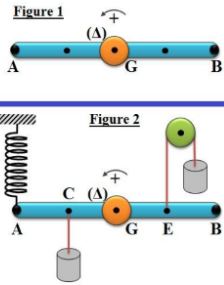
\includegraphics[width=0.25\textwidth]{./img/ex04.png}
  \end{center}
\end{wrapfigure}

On considère une barre rigide et homogène de longueur $L = AB$
pouvant tourner autour d'un axe horizontal fixe ($\Delta$) passant au
centre d'inertie G où elle est en équilibre lorsqu’elle est en
position horizontale. (Figure 1)

\begin{enumerate}
\item Faire l’inventaire des forces appliquées à la barre (AB).
\item  Rappeler les conditions d’équilibre de la barre (AB).

	Par deux fils, on applique deux forces $\vec{F_1}$ et $\vec{F_2}$ de même intensité
	$F=2N$. En appliquant une force $\vec{T}$ par un ressort pour garder la
barre (AB) en équilibre horizontal. (Figure 2)

\item  Les forces $F_1$ et $F_2$ forment-elles un couple de forces?

\item  Déduire la valeur de T tension du ressort.
\item  En utilisant la méthode géométrique, déduire la valeur de R
l'intensité de la force appliquée par l'axe ($\Delta$) sur la barre (AB).
\end{enumerate}

\textbf{Données:} $P = 3N$; $CG = EG = \frac{L}{4}$ ; L'échelle $1N \rightarrow 1cm$.


\end{Box2}
%%%_________________________Exercice 6 : _________________________Exercice

\begin{Box2}{Exercice 6 :Couple de Torsion }


On fixe au centre de gravité G d'une barre homogène (AB) de longueur $L = 50cm$, un fil de torsion de
constante de torsion C.

On fixe l'extrémité A à un ressort de raideur $K = 50N/m$ et l'extrémité B
à un fil vertical qui porte à l'autre extrémité un solide (S) de masse
$m=200g$.
	\begin{wrapfigure}[4]{r}{0.28\textwidth}
  \begin{center}
	  \vspace{-2cm}
	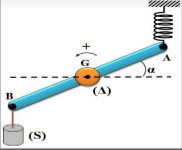
\includegraphics[width=0.28\textwidth]{./img/ex05.png}
  \end{center}
\end{wrapfigure}
A l'équilibre le fil de torsion est tordu d'un angle $\alpha$ = 30° et le ressort est
vertical et allongé de $\Delta{L} = 4cm$.

\begin{enumerate}

	\item  Montrer que les tensions du ressort et du fil forment un couple de deux
forces.
\item  Calculer la valeur de la constante de torsion C.
\end{enumerate}

\end{Box2}


\begin{Box2}{Exercice 7 : Equilibre d’un solide sans et avec frottement  }
	\begin{wrapfigure}[4]{r}{0.28\textwidth}
  \begin{center}
	  \vspace{-0.9cm}
	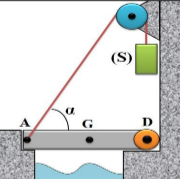
\includegraphics[width=0.28\textwidth]{./img/ex06.png}
  \end{center}
\end{wrapfigure}

On veut soulever le pont-levis à l'aide du corps (S) qui exerce une force de traction $\vec{T}$ sur le pont. La longueur du pont   $L$=$DA$=$6 m$, sa masse
$M=800kg$ et l'angle $\alpha$ = 40°, avec g = 10N/kg.

\begin{enumerate}

	\item  Donner l'expression du moment de toutes les forces appliquées sur le
pont à l'équilibre lorsque le pont est horizontal.
\item  Déterminer l’intensité T et la masse m du corps (S).
\item  Déterminer par la méthode analytique la force de réaction $\vec{R}$ exercée
par l’axe de rotation en D contre le pont, ainsi que l’angle $\beta$ que cette
force forme avec l’horizontale.
\end{enumerate}

\end{Box2}



\begin{Box2}{Exercice 8 : Equilibre d’un solide  }
	\begin{wrapfigure}[4]{r}{0.28\textwidth}
  \begin{center}
	  %\vspace{-0.9cm}
	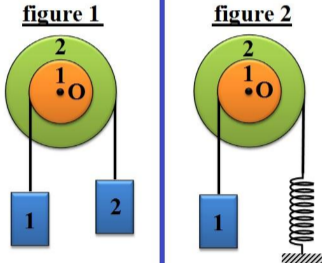
\includegraphics[width=0.28\textwidth]{./img/ex07.png}
  \end{center}
\end{wrapfigure}

Le dispositif représenté par la (figure 1) comprend :

\begin{itemize}
	\item  Une poulie à deux gorges pouvant tournées
sans frottement autour d'un axe fixe $(\Delta)$
horizontal passant par le point O.
\item Deux fils $(f_1)$ et $(f_2)$ fixés respectivement aux
gorges, enroulés sur celles-ci et supportant les
masses $m_1$ et $m_2$.
\end{itemize}

\begin{enumerate}

	\item Rappeler les conditions d'équilibre d'un solide
pouvant tourné \\ autour d'un axe fixe.

\item  Donner l'expression du moment de chaque force.

\item Calculer $m_2$ pour que le dispositif soit en
équilibre.

On remplace la masse $m_2$ par un ressort de raideur $k = 20N/m$ dont l'extrémité inférieure est fixée.
(figure2)

\item  Calculer l'allongement du ressort à l'équilibre du système.
\end{enumerate}

\textbf{Données:} $m_1 = 120g$; $r_1 = 10cm$ et $r_2 = 15cm$; $g = 9,8 N/kg$.

\end{Box2}





\begin{center}
	\emph{Excuses make today easy, but tomorrow harder --- Discipline makes today hard, but tomorrow easier }


	\emph{\textbf{Future Is Loading...}}

\end{center}

\end{document}
